\section{State Machines}

\frame{
{Part 2: State Machines}

\tableofcontents[currentsection,hideallsubsections, firstsection=2, sections={2-4}]
}

\subsection{Definition}

\begin{frame}{What are state machines?}

  State machines are used to represent "step-by-step" processes. They contain:
  \begin{itemize}
    \item A description of each possible state in the machine;
    \item How the machine transition from one state to another;
  \end{itemize}\bigskip

  State machines are often used to describe algorithms, programs, logic circuit, decision processes, etc.\bigskip

  State machines are a \structure{formal description} that can be used to prove the correctness of an algorithm.
\end{frame}

\begin{frame}[t]{Example of a State Machine}

  \begin{columns}
    \column{0.4\textwidth}
    State machine for counting from 0 to 99:
    \begin{itemize}
      \item {\bf States:} 0 to 99, overflow.
      \item {\bf Start State:} 0
      \item {\bf Transitions:}\\
        $i \to i+1$ if $i < 99$\\
        $99 \to$ overflow\\
        overflow $\to$ overflow\\
    \end{itemize}\bigskip

    Note how we can represent the State Machine many different ways.

    \column{0.6\textwidth}
    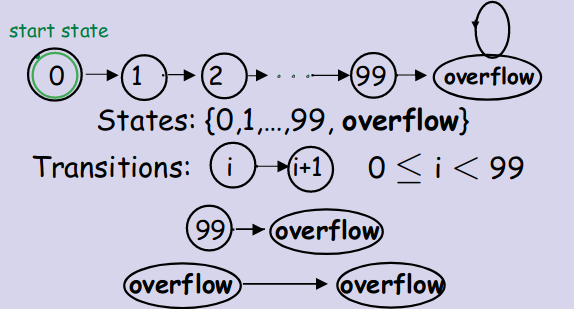
\includegraphics[width=1\textwidth]{../img/statemachine}
  \end{columns}
\end{frame}

\subsection{State Machines for Proofs}
\begin{frame}{State Machine for Proofs}{Robot 1.0}

  Imagine a robot moving forwards and backwards on a street. The robot has two speeds:
  \begin{itemize}
    \item The robot can move exactly {\bf five squares} forwards.
    \item The robot can move exactly {\bf three squares} backwards.
  \end{itemize}
  \bigskip

  If the robot starts from position 0, is it possible for it to reach position 4?
\end{frame}

\begin{frame}{State Machine for Proofs}{Robot 1.1}
  Imagine a robot moving forwards and backwards on a street. The robot has two speeds:
  \begin{itemize}
    \item The robot can move exactly {\bf nine squares} forwards.
    \item The robot can move exactly {\bf three squares} backwards.
  \end{itemize}
  \bigskip

  If the robot starts from position 0, is it possible for it to reach position 4?
\end{frame}

\begin{frame}{State Machine for Proofs}{Preserved Invariants}

  \structure{Preserved Invariants} are propositions that are always true, after {\bf any} transition of the state machine. We can use preserved invariants to prove which squares the robots can reach.

  \begin{block}{Robot 1.0}
    The position of robot 1.0 is always: $s_0 + 5a - 3b$
  \end{block}
  \begin{block}{Robot 1.1}
    The position of robot 1.1 is always: $s_0 + 9a - 3b$
    \begin{itemize}
      \item $s_0 + 9a - 3b = s_0 + 3(3a-b)$
      \item The position of robot 1.1 is always $s_0$ plus a multiple of 3; (\structure{Preserved Invariant})
      \item So it is impossible for robot 1.1 to reach 4 from 0.
    \end{itemize}
  \end{block}
\end{frame}


\begin{frame}{Induction with Preserved Invariants}

  Preserved Invariants can be used together with inductions to prove things about state machines:\bigskip

  \begin{itemize}
    \item Prove that $P(s)$ is a preserved invariant. This means that if $P(s)$ is true for some state $s$, then it will continue to be true after any transition.\medskip

    \item Prove that $P(s)$ is true for the initial state, $s_0$.\medskip

    \item Conclude that $P(s)$ is always true for the entire state machine.
  \end{itemize}\bigskip

  If $P(s)$ is a "correctness condition" of an algorithm, this method can be used to prove that an algorithm is correct.
\end{frame}


\begin{frame}{State Machine for Proofs}{Robot 2.0}

  Robot 2.0 can move on the diagonals of $\mathbb{Z}^2$: (+1,
  +1), (-1,-1), (+1,-1), (-1,+1). Starting from (0,0), is it possible for the robot to reach position (1,0)?

  \begin{center}
    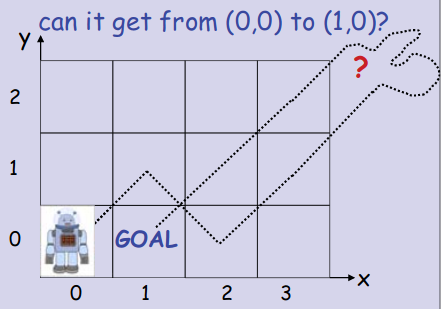
\includegraphics[width=0.4\textwidth]{../img/diag_robot}
  \end{center}

  \alert{QUIZ}: Try to prove this by yourself first!

\end{frame}


\begin{frame}{State Machine for Proofs}{Robot 2.0 -- Solution}

  We can show that a \structure{preserved invariant} of robot 2.0 is that the sum of its coordinates is always even (or always odd):\bigskip

  \begin{itemize}
  \item P(0,0) is true (0+0 is even).
  \item The steps of the robot are:
    \begin{itemize}
    \item $+1+1 = +2$: even + 2 is still even;
    \item $-1-1 = -2$: even - 2 is still even;
    \item $+1-1 = 0$: even + 0 is still even;
    \item $-1+1 = 0$: even + 0 is still even;
    \end{itemize}
  \end{itemize}
  \bigskip

  So we can see that the parity of the position is a \structure{preserved invariant}. Because the parities of (0,0) and (1,0) are different, it is impossible for robot 2.0 to go from (0,0) to (1,0).
\end{frame}

\begin{frame}{State Machines for Proofs}{Fast Exponentiation}

  This is the end for this lecture. I highly recommend that you watch lecture video 1.9.1 from MIT OCW for a final example with the Fast Exponentiation algorithm.\bigskip

  Summary of the third part: To prove that an algorithm is correct, we need to show that:
  \begin{itemize}
    \item Prove that if the algorihm is in a correct state, it will always stay in the correct state (preserved invariant);
    \item Prove that the algorithm can reach the correct state from the initial position;
    \item Prove that the algorithm stops at some point (not an infinite loop).
    \begin{itemize}
      \item We haven't talked about this part yet, but you can prove this by showing that some variable in the state machine is always decreasing.
    \end{itemize}
  \end{itemize}
\end{frame}
